\documentclass[10pt,landscape,a4paper]{article}
\usepackage[landscape]{geometry}
\usepackage{multicol}
\usepackage{ifthen}
\usepackage{hyperref}
\usepackage{listings}
\usepackage{graphicx}
\usepackage{color}
\lstset{numbers=left, xleftmargin=0.5cm, xrightmargin=0.5cm}

% Template is based on work of 2014 Winston Chang
% see: https://github.com/wch/latexsheet

\ifthenelse{\lengthtest { \paperwidth = 11in}}
	{ \geometry{top=.5in,left=.4in,right=.4in,bottom=.5in} }
	{\ifthenelse{ \lengthtest{ \paperwidth = 297mm}}
		{\geometry{top=1cm,left=1cm,right=1cm,bottom=1cm} }
		{\geometry{top=1cm,left=1cm,right=1cm,bottom=1cm} }
	}


\pagestyle{empty}                 % dont need any header or footer
\setcounter{secnumdepth}{0}  % dont need section numbering

% Redefine section commands to use less space
\makeatletter
\renewcommand{\section}{\@startsection{section}{1}{0mm}%
                                {-.8ex plus -.5ex minus -.2ex}%
                                {0.5ex plus .2ex}%x
                                {\normalfont\large\bfseries}}
\renewcommand{\subsection}{\@startsection{subsection}{2}{0mm}%
                                {-.8explus -.5ex minus -.2ex}%
                                {0.5ex plus .2ex}%
                                {\normalfont\normalsize\bfseries}}
\renewcommand{\subsubsection}{\@startsection{subsubsection}{3}{0mm}%
                                {-.8ex plus -.5ex minus -.2ex}%
                                {1ex plus .2ex}%
                                {\normalfont\small\bfseries}}
\makeatother

\setlength{\parindent}{0pt}
\setlength{\parskip}{0pt plus 0.5ex}


% -----------------------------------------------------------------------

\begin{document}

\raggedright
\footnotesize
\begin{multicols}{2}

% multicol parameters
\setlength{\premulticols}{1pt}
\setlength{\postmulticols}{1pt}
\setlength{\multicolsep}{3pt}
\setlength{\columnsep}{2pt}

\begin{center}
     \Large{\textbf{Java Basics Course - Lesson 1}} \\
\end{center}

\section{Java}
\begin{tabular}{@{}ll@{}}
\verb!JRE!  & Java Runtime Environment \\
\verb!JDK!  & Java Development Kit\\
\verb!JVM!  & Java Virtual Machine\\
\verb!JAVA_HOME! & Location where a JRE or JDK is installed\\
\end{tabular}\\
Java programs are compiled to byte code which requires the Java Virtual machine to run. The byte code is portable and can be executed in JVMs running on different hardware (e.g. x86, ARM). 

\section{File Types}
\begin{tabular}{@{}ll@{}}
\verb!*.java!    & Text files containing the Java source code. \\
\verb!*.class!  & Contains the bytecode to be executed by JVM.  \\
\verb!*.jar! & A Java archive file, basically a zip-archive. \\
\verb!MANIFEST.mf!  & Describes dependencies and main class.  \\
\end{tabular}\\
Java classes are packaged into JAR files which also contain a description in META-INF/MANIFEST.mf. The manifest describes the dependencies and the main entry point to launch the program.

\section{A First Example}
\subsection{Steps to writing the program: \texttt{HelloDuke.java}}
\newlength{\MyLen}
\settowidth{\MyLen}{\texttt{letterpaper}/\texttt{a4paper} \ }
\begin{itemize}
\item create new directory and cd into it \texttt{lesson-01/src}.
\item create a new file \texttt{HelloDuke.java}.
\item edit \texttt{HelloDuke.java} and enter follwing code:
\end{itemize}
\lstinputlisting[language=Java,frame=single,firstline=1, lastline=7]{../src/HelloDuke.java}

\subsection{Compiling and running the program}
Java programs need to be compiled before starting them. Unlike with R, Java code cannot be executed directly. Run following code on a command line interface (CLI) to compile and run the code in \texttt{HelloDuke.java}.
\begin{lstlisting}[language=bash,frame=single]
> javac HelloDuke.java
> java HelloDuke
Want some coffee?

\end{lstlisting}
\begin{tabular}{@{}ll@{}}
\verb!javac!  & The Java compiler, translates source code into byte code.\\
\verb!java!  & Launches the JVM with the given class.\\
\end{tabular}\\

\subsection{Packaging the program - creating a JAR}
Java programs are not distributed by class files, instead archives are used where all required class files are collected within one JAR file. With Java 8 a plain JAR file is created with:
\begin{lstlisting}[language=bash,frame=single]
# Java 8
> jar cf HelloDuke.jar HelloDuke.class

# Java 9
> jar --create --file HelloDuke.jar HelloDuke.class
\end{lstlisting}

\subsection{Creating a runnable JAR}

As the JVM requires an information about which class to launch, executing this JAR file will result in an error.
\begin{lstlisting}[language=bash,frame=single]
> java -jar HelloDuke.jar
kein Hauptmanifestattribut, in Hello.jar
\end{lstlisting}
It is possible to define a list of JAR files (separated by ;) using the \texttt{-classpath} argument.
\begin{lstlisting}[language=bash,frame=single]
> java HelloDuke -classpath Hello.jar;
Want some coffee?

\end{lstlisting}
It is also possible to point to a directory using the  \texttt{-cp} argument where  \texttt{-cp .} refers the current directory.
\begin{lstlisting}[language=bash,frame=single]
> java HelloDuke -cp .
Want some coffee?

\end{lstlisting}
The JAR command allows to define an entry point, the so called main class. 
\begin{lstlisting}[language=bash,frame=single,breaklines=true]
# Java 8 
> jar cfe HelloDuke.jar HelloDuke HelloDuke.class

# Java 9 
> jar --create --main-class=HelloDuke --file HelloDuke.jar HelloDuke.class
\end{lstlisting}

\subsection{Executing a runnable JAR}
A runnable JAR can be launched on command line using the \texttt{java} command. It is no longer needed to specify the classpath or the main class.  
\begin{lstlisting}[language=bash,frame=single]
> java -jar HelloDuke.jar
Want some coffee?

\end{lstlisting}
Lets extract the JAR file and have a look at the \texttt{META-INF/MANIFEST.mf} file which was created during the package process:
\begin{lstlisting}[language=bash,frame=single]
# Java 8
> jar xf HelloDuke.jar
# Java 9
> jar -xf HelloDuke.jar
\end{lstlisting}
After extraction, listing \texttt{MANIFEST.mf} will reveal main class definition, which causes the JVM to find the proper entry point to launch the \texttt{HelloDuke.class}. Compiled with Java 8 the manifest file will look like:
\begin{lstlisting}[language=bash,frame=single]
# on Windows command line one could use:
> type META-INF\MANIFEST.MF
# on a Bash shell:
> cat META-INF/MANIFEST.MF
Manifest-Version: 1.0
Created-By: 1.8.0_152 (Oracle Corporation)
Main-Class: HelloDuke
\end{lstlisting}
Beside the manifest, \texttt{HelloDuke.jar} contains a single file only, it is\texttt{HelloDuke.class}. The entry \texttt{Main-Class: HelloDuke} directly points to this single class file.

\section{Creating an Eclipse project}
\subsection{Setting up a new project}
\begin{multicols}{2}
With the first start, Eclipse will ask you for a workspace location. A workspace is intended to contain one ore more projects. It can be any folder you like. When there are multiple workspaces, Eclipse will ask which workspace to open. Multiple instances of Eclipse can be started but a workspace can only opened by one Eclipse instance.\\
\begin{itemize}
\item Go to menu: \texttt{File / New Java Project}.
\item Enter new project name \texttt{HelloDuke}.
\item Ensure that in project layout, the option to create separate folders for sources and classes is set. 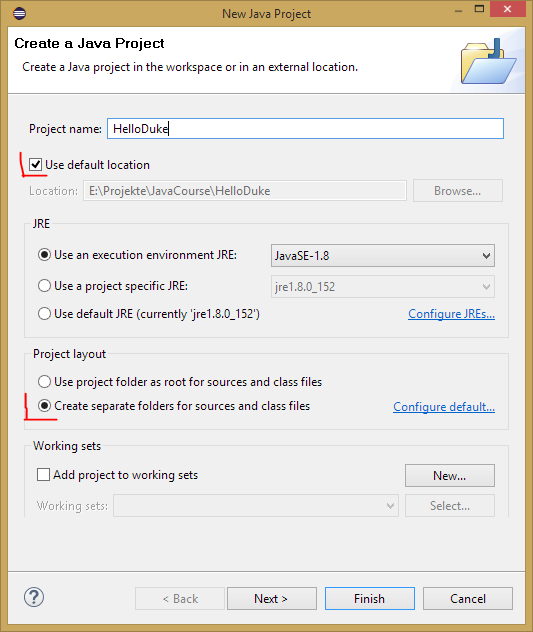
\includegraphics[width=.9\linewidth]{../slides/EclipseProjectWizard1.png}\\
\item Continue with next.
\item Review project layout and click finish. 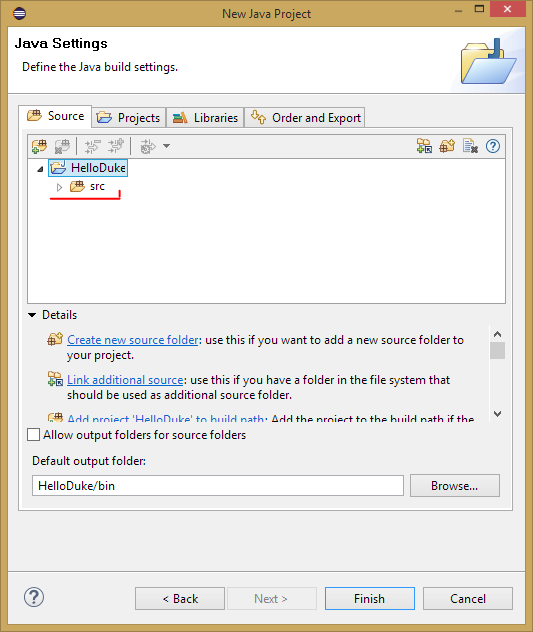
\includegraphics[width=1\linewidth]{../slides/EclipseProjectWizard2.png}
\end{itemize}
The new project will appear as follows in Eclipse Project Navigator.

\includegraphics[width=.9\linewidth]{../slides/EclipseProjectExplorerNewProject1.png}
\end{multicols}
\subsection{Creating and running the first Java program}
Selecting thr project root and opening the context menu, new objects can be created. So here a new class with the name \texttt{HelloDuke} can be created.\\
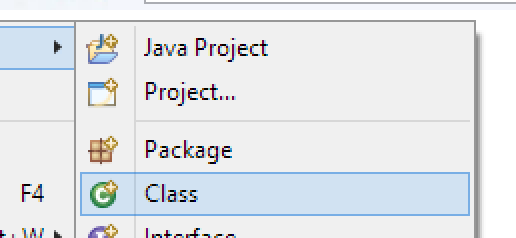
\includegraphics[width=.3\linewidth]{../slides/ContextMenu_CreateClass.png} 
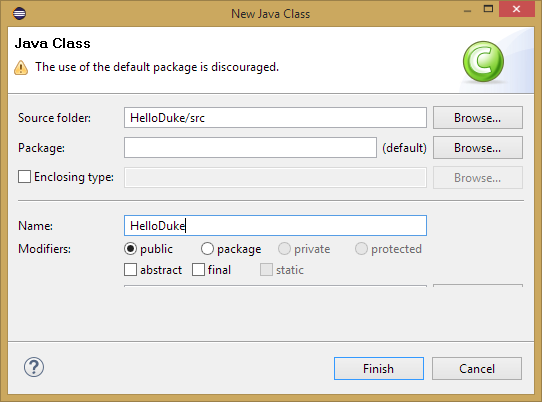
\includegraphics[width=.5\linewidth]{../slides/EclipseProjectExplorerNewClass2.png}\\
As soon as the class was created it can be edited in Eclipses Java code editor. The editor offers powerful code completion. As the main class skeleton was created automatically, it is sufficient to just type \texttt{main} and then press \texttt{CTRL}+\texttt{SPACE} to bring up code completion. Eclipse will offer automatic creation of a static main method, which is required to execute the program. Double click or just pressing \texttt{RETURN} or \texttt{ENTER} will insert the code.\\
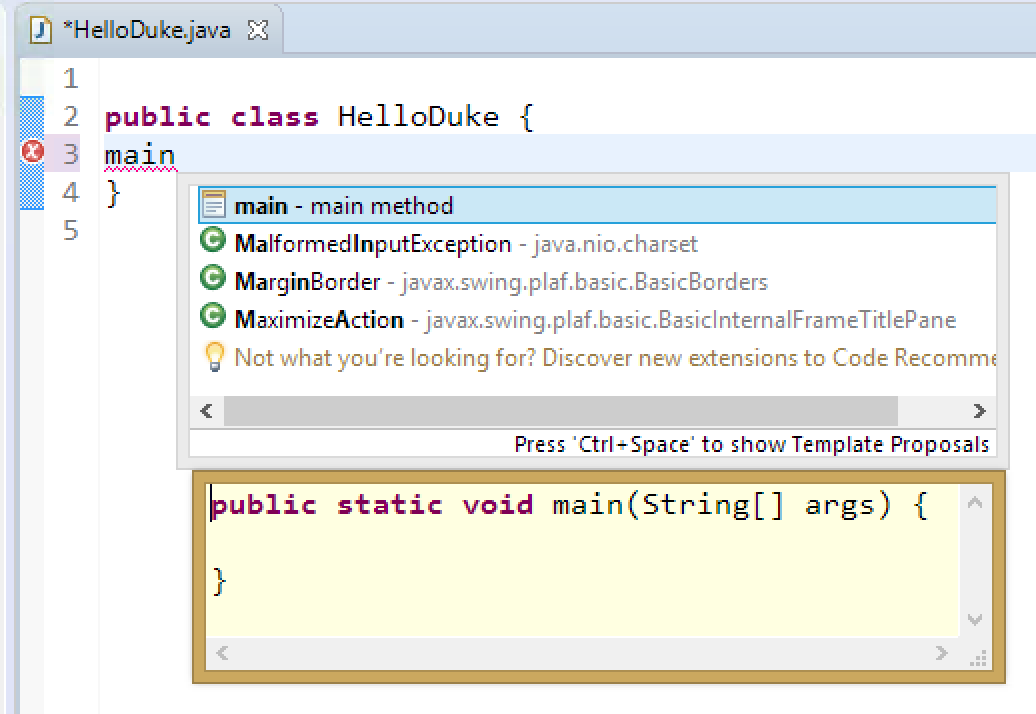
\includegraphics[width=.5\linewidth]{../slides/CodeCompletion_MainMethod.png}\\
After completing the code as in the example, the program can be launched either using context menu on \texttt{HelloDuke.java} or via manual configuration. Here program execution via context menu is shown.\\
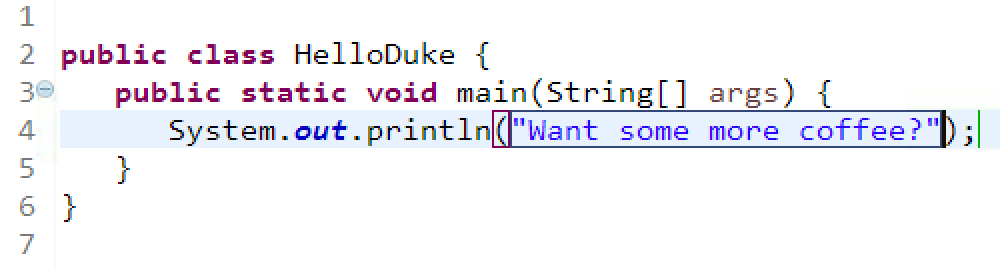
\includegraphics[width=.7\linewidth]{../slides/CodeEditor_HelloDukeCode.png}\\
One should note, that \texttt{HelloDuke.java} is located inside the \texttt{Default Package}. Packages are an essential concept and are covered in Lesson 2.\\
\begin{multicols}{2}
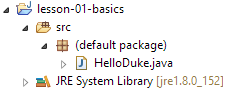
\includegraphics[width=.81\linewidth]{../slides/EclipseProjectExplorerDefaultPackage.png}\\
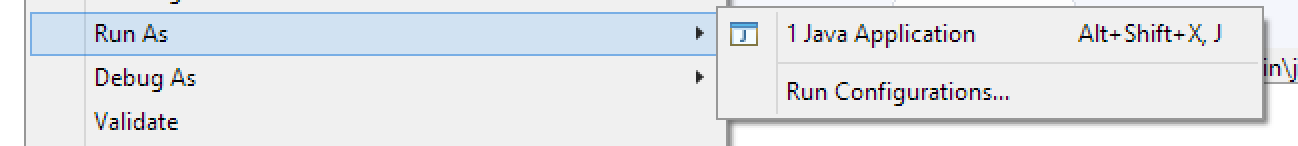
\includegraphics[width=1\linewidth]{../slides/ContextMenu_Project_RunAs.png}\\
\end{multicols}
Select \texttt{HelloDuke.java} then open the context menu, go to \texttt{Run As} then select \texttt{1 Java Application}. The program will be executed and the console view will show the desired result.\\
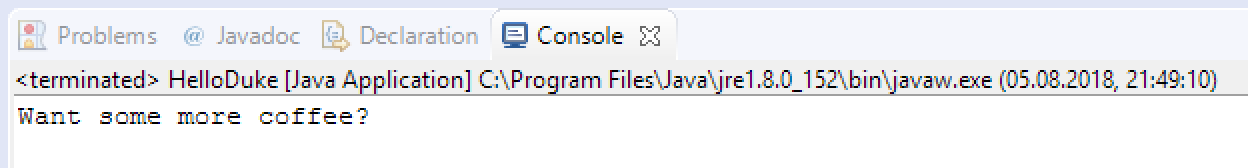
\includegraphics[width=.8\linewidth]{../slides/ConsoleWindow_WantMoreCoffee.png}
After first execution of \texttt{HelloDuke.java} a \texttt{Run Configuration} is created. This configuration can be reused for repeated execution and for JAR file creation.
\subsection{Exporting a runnable JAR}
\begin{itemize}
\item Select the project root and open its context menu OR open the file menu - in both cases select the \texttt{Export} command.
\item Then select the \texttt{Runnable JAR file} from \texttt{Java} section, continue with \texttt{next.}
\item There will be one launch configuration with the name \texttt{HelloDuke - HelloDuke}.
\item An \texttt{export destination} must be provided, usually the project root folder with a suitable name such as \texttt{lesson-01-basics/HelloDuke.jar}.
\item Click on \texttt{Finish} and verify that the JAR file starts (double click on Windows or just run java command on command line).
\end{itemize}
\end{multicols}
\end{document}